\documentclass[conference]{IEEEtran}
\usepackage[utf8]{inputenc}
\usepackage{csquotes}
\usepackage[spanish]{babel}
%\decimalpoint
\usepackage{amsmath,amssymb,amsfonts}
\usepackage{graphicx}
\usepackage{hyperref}
\usepackage{float}
\usepackage{graphicx}
\usepackage{lmodern}
\usepackage{amsmath}
\usepackage[per-mode=fraction, inter-unit-product=\cdot]{siunitx}

\allowdisplaybreaks
\graphicspath{{./images}}
\makeatletter
\makeatother
\usepackage{listings}
\lstset{language=Python}

\usepackage[style=ieee]{biblatex}
\renewbibmacro*{bbx:savehash}{} % Quita rayas para autores repetidos
\addbibresource{references.bib}
\def\BibTeX{{\rm B\kern-.05em{\sc i\kern-.025em b}\kern-.08em
    T\kern-.1667em\lower.7ex\hbox{E}\kern-.125emX}}

\hyphenation{op-tical net-works semi-conduc-tor} % cómo partir palabras en cambios de línea

\newcolumntype{M}[1]{>{\centering\arraybackslash}m{#1}}

\pagestyle{plain}

\makeatletter
\newcommand{\linebreakand}{%
  \end{@IEEEauthorhalign}
  \hfill\mbox{}\par
  \mbox{}\hfill\begin{@IEEEauthorhalign}
}


\title{µwgpu: Herramientas de Microbenchmarking de GPU Multiplataforma}

\author{\IEEEauthorblockN{Ignacio Vargas Campos}
\IEEEauthorblockA{\textit{Ingeniería en Computadores} \\
\textit{Instituto Tecnológico de Costa Rica}\\
Cartago, Costa Rica \\
ignacio.vargas@estudiantec.cr}
}
\begin{document}

\markboth{IEEE, Proyecto 2, Arquitectura de computadora}{ \MakeLowercase{\textit{et al.}}: Tecnológico de Costa Rica}

\maketitle
\thispagestyle{plain}

\begin{abstract}

El presente trabajo introduce µwgpu, una infraestructura multiplataforma para
el benchmarking de GPUs que utiliza tecnologías emergentes como WebGPU. Esta
solución incluye:

\begin{enumerate}
  \item Una biblioteca modular para facilitar la creación de microbenchmarks.
  \item Un banco de microbenchmarks enfocado en operaciones computacionales comunes y rendimiento de memoria.
  \item Herramientas de interacción web y de línea de comandos para maximizar su accesibilidad.
\end{enumerate}

El proyecto aborda las limitaciones de herramientas existentes al ofrecer una
alternativa abierta para ejecución multiplataforma de microbenchmarks. Aunque
se identificaron áreas de mejora, como la optimización avanzada y la
inclusión de datos de entornos nativos, µwgpu establece un marco innovador
que potencia la colaboración y la investigación en el ámbito de GPUs.

\end{abstract}

\section{Introducción}

Las GPUs son piezas clave en el avance de aplicaciones computacionales intensivas, como el aprendizaje automático y la visualización en tiempo real. Sin embargo, las rápidas actualizaciones en los diseños y la falta de transparencia en los detalles microarquitectónicos por parte de los fabricantes dificultan el análisis y la optimización del rendimiento. Herramientas específicas como CUDA han permitido explorar características arquitectónicas, pero debido a su naturaleza cerrada y dependencia del hardware limita su alcance.

Desarrolladores e investigadores desean optimizar y entender el rendimiento de programas para GPUs en diferentes plataformas.
El entendimiento necesario para poder realizar estas optimizaciones requiere
información detallada sobre el rendimiento del hardware en múltiples
plataformas. Aunque ha habido estudios en esta área, muchos se han
especializado en hardware de NVIDIA, dejando a los desarrolladores de
plataformas generales sin la información que necesitan (TODO referencias).
Esto representa un desafío para asegurar que las aplicaciones funcionen de
manera eficiente en todas las plataformas y hace más difícil identificar
problemas de rendimiento o bugs en las distintas capas (desde APIs hasta el
hardware), lo cual es crucial tanto para la investigación como para los
productos comerciales.

Este proyecto, µwgpu (micro wgpu), se presenta como una solución integral y
moderna, que aprovecha tecnologías como WebGPU y wgpu para proporcionar un
marco multiplataforma para el microbenchmarking de GPUs.
El objetivo principal es crear la infraestructura necesaria para simplificar la
ejecución de pruebas de rendimiento y recolección de datos así como
proporcionar un banco de microbenchmarks para operaciones comunes realizadas en
GPUs.

Cabe aclarar que el alcance de µwgpu se delimita a proporcionar las
herramientas y el marco para facilitar la medición del rendimiento de GPUs en
diferentes plataformas, sin entrar en una recolección de datos exhaustiva ni el
análisis detallado de estos.
Este enfoque busca democratizar el acceso a las pruebas de rendimiento,
permitiendo una evaluación más inclusiva y diversificada de las capacidades
gráficas en diferentes contextos.

\section{Antecedentes}

El estudio del rendimiento de las unidades de procesamiento gráfico (GPUs) a
nivel granular ha sido objeto de interés académico e industrial debido a su
impacto en el diseño de software y hardware. Sin embargo, esta área enfrenta
limitaciones tanto en términos de herramientas como de estándares
multiplataforma para microbenchmarking \cite{muniyappamicro}.

\subsection{Microbenchmarks en GPUs y CUDA}

El análisis de microarquitectura de GPUs se ha centrado históricamente en
herramientas específicas como CUDA, una API cerrada desarrollada por NVIDIA que
facilita el desarrollo y ejecución de programas en sus dispositivos. Estudios
como el de Mei y Chu han explorado características como la jerarquía de memoria
de las GPUs mediante microbenchmarks de bajo nivel, destacando la relevancia de
optimizar el acceso a la memoria global y compartida \cite{mei2016dissectinggpumemoryhierarchy}. Por otro lado, trabajos
como el de Wong et al. se han enfocado en desmitificar la microarquitectura de
GPUs para mejorar la modelización y el rendimiento del software \cite{wong2010demystifying}. Sin embargo,
estas y muchas investigaciones están inherentemente limitadas a arquitecturas y
APIs específicas, como CUDA, restringiendo su aplicabilidad en plataformas no
compatibles \cite{jia2018dissecting} \cite{jia2019dissecting} \cite{luo2024benchmarking} \cite{anzt2020evaluating} \cite{abdelkhalik2022demystifying}.

\subsection{Limitaciones en esfuerzos anteriores}

A pesar de estos avances, los estudios existentes presentan importantes
restricciones. Herramientas como CUDA están diseñadas exclusivamente para
hardware de NVIDIA, excluyendo otras plataformas como AMD o Intel, y los métodos
propuestos a menudo carecen de estándares para la comparación cruzada. Por
ejemplo, los microbenchmarks de memoria analizados por Wong revelaron
características ocultas de la jerarquía de memoria en GPUs específicas, pero no
ofrecen soluciones multiplataforma \cite{wong2010demystifying}.

En este contexto, han habido pocas iniciativas de explorar el rendimiento a
fondo fuera del hardware de NVIDIA, uno de los pocos ejemplos de proyectos que
han buscado este tipo de exploración es el proyecto µVkCompute de Google
\cite{uVkCompute}. Este proyecto ha intentado abordar estas limitaciones al
enfocarse en la API Vulkan, que permite benchmarks en plataformas y hardwares
más amplios pero carece de estudios formales y estandarización
\cite{devon2024gpuperformancemodelingmicrobenchmarks}, además de que Vulkan no
tiene soporte en todas las plataformas notando aquellas de la compañía Apple o
lo navegadores web.

\subsection{Avances recientes: WebGPU y wgpu}

El surgimiento de WebGPU representa un cambio paradigmático en el desarrollo
gráfico. Este estándar, respaldado por el W3C, permite ejecutar programas
gráficos en navegadores sobre cualquier plataforma y hardware compatible,
eliminando muchas de las barreras tradicionales de compatibilidad \cite{webgpu}.


La biblioteca wgpu, es una implementación de WebGPU desarrollada para Firefox,
pero también tiene capacidades extendidas de usarse como su propio API gráfico
que puede compilarse para navegadores (utilizando WebGPU por debajo) o para
programas nativos (utilizando cualquier driver disponible como Vulkan, Metal o
D3D12) \cite{wgpu} \cite{devon2024gpuperformancemodelingmicrobenchmarks}. Esto
significa que el API gráfico wgpu permite crear programas (y a nuestro interés
microbenchmarks) de una manera multiplataforma que no se había logrado antes.

\section{Descripción de la solución desarrollada}

Ante estas limitaciones y oportunidades, el proyecto µwgpu, inspirado en
µVkCompute, establece un marco e infraestructura multiplataforma para el
análisis granular de rendimiento de GPUs a través de microbenchmarks
\cite{uVkCompute}. Esto aborda la falta de herramientas generalizadas, y a
futuro se podría utilizar para responder a la necesidad de estudios
sistemáticos en plataformas y arquitecturas diversificadas, contribuyendo al
estado del arte y fomentando mejores prácticas en el diseño y optimización de
software gráfico \cite{devon2024gpuperformancemodelingmicrobenchmarks}.

Se escogió utilizar wgpu para desarrollar el software de microbenchmarks debido a su ya mencionado gran alcance multiplataforma.
En la figura \ref{fig:wgpu_plataformas} se muestra el alcance de esta API gráfica y cómo accesa el hardware a través de los diferentes APIs gráficos y sistemas operativos.

\begin{figure}
  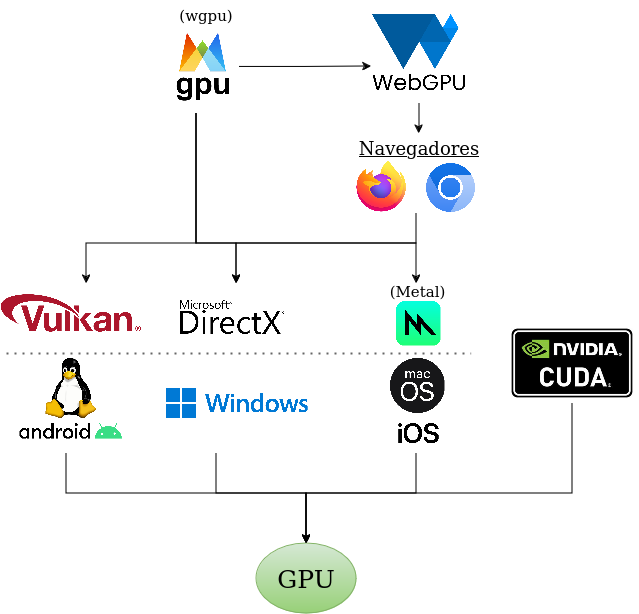
\includegraphics[width=1.05\linewidth]{images/Diagrama Plataformas.png}
  \caption{Plataformas a través de las cuales wgpu actúa sobre el hardware.
  Nótese que CUDA no es un driver que puede utilizar wgpu, ya que es sumamente
  especializado y solo se utiliza para hardware de NVIDIA.}
  \label{fig:wgpu_plataformas}
\end{figure}

Para tener una solución holística para crear y ejecutar microbenchmarks en todas las plataformas posibles así como recolectar datos de rendimiento se desarrollaron los siguientes productos de software:

\begin{enumerate}
  \item Una biblioteca para simplificar la elaboración de microbenchmarks de wgpu. A esta se le llamó “uwgpu”.
  \item Un banco de microbenchmarks creado usando “uwgpu” para evaluar
    múltiples operaciones computacionales comúnmente implementadas en GPU así
    como algunas características de su memoria.
  \item Un programa de CLI para ejecutar los microbenchmarks.
  \item Un servidor web que sirve una página en la que los usuarios pueden
    correr los microbenchmarks en su computador y enviar sus resultados a una
    base de datos para crear un banco de datos de rendimiento.
\end{enumerate}

Estos productos se escogieron para cumplir con los casos de uso definidos para
la solución, los cuales se
presentan en la figura \ref{fig:casos_de_uso}.

\begin{figure}
  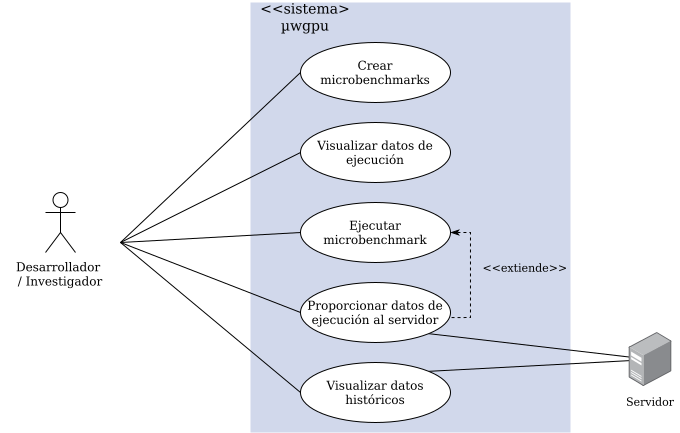
\includegraphics[width=\linewidth]{images/UML Casos de Uso.png}
  \caption{Diagrama UML de los casos de uso definidos para la solución.}
  \label{fig:casos_de_uso}
\end{figure}

A continuación se describe cada elemento en mayor detalle.

\subsection{Biblioteca principal uwgpu}

Esta biblioteca responde a la necesidad de poder crear microbenchmarks de una
manera multiplataforma. Simplifica el proceso de crear microbenchmarks
utilizando wgpu, para reducir el código repetitivo que requiere cualquier
aplicación que utilice el API gráfico. También se encarga de medir los tiempos
de ejecución y ejecutar las repeticiones de la operación que se esté midiendo
la cantidad de veces indicada.

El diagrama de la figura \ref{fig:diagrama_clases} muestra las clases de la biblioteca “uwgpu” para crear microbenchmarks.
Muestra las clases expuestar por esta API y cómo se componen.
Aquellos tipos que no se especifican en el diagrama es porque son propios del lenguaje Rust o propios del API gráfico wgpu.

\begin{figure}
  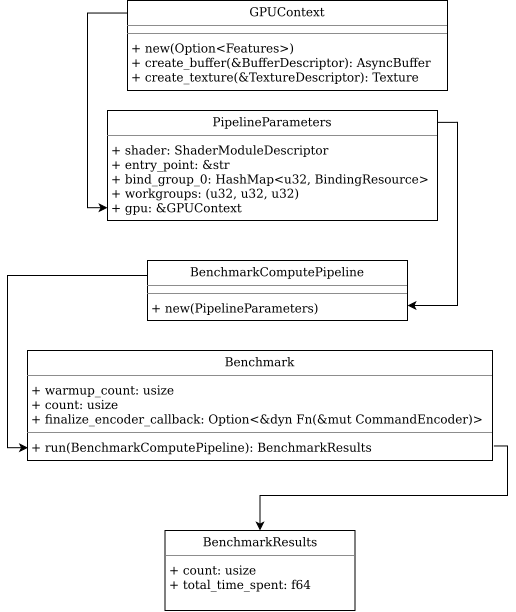
\includegraphics[width=\linewidth]{images/Clases uwgpu.png}
  \caption{Diagrama UML de clases para biblioteca “uwgpu”.}
  \label{fig:diagrama_clases}
\end{figure}

En líneas generales, un usuario de esta biblioteca primero obtiene una
referencia al dispositivo GPU creando un “GPUContext”. Con esto puede
crear un pipeline computacional creando un “BenchmarkComputePipeline”
pasando los parámetros necesarios como el shader (operación gráfica) que desea
evaluar y otros parámetros que requiere para ejecutar. Finalmente con este
pipeline define el “Benchmark” a ejecutar, la biblioteca se encarga de
ejecutarlo tomando en cuenta aspectos detallados del API gráfico que abstrae y
finalmente devuelve los resultados de la ejecución en el objeto
“BenchmarkResults”.

\subsection{Banco de microbenchmarks}

Utilizando la biblioteca uwgpu se crearon microbenchmarks para las siguientes
operaciones computacionales comunes:

\begin{enumerate}
  \item Multiplicación Matricial
  \item Convolución
  \item Reducción (suma)
  \item Scan (suma de prefijos)
\end{enumerate}

También se crearon microbenchmarks para medir el rendimiento de la memoria en
los siguientes aspectos:

\begin{enumerate}
  \item Copiar memoria entre buffers
  \item Copiar memoria de un buffer a una textura
  \item Copiar memoria entre texturas
\end{enumerate}

Todos estos microbenchmarks se hicieron disponibles como una biblioteca aparte
que es utilizada por los componentes de interfaz del proyecto. Se creó tomando
en cuenta que fuera compilable a Web Assembly para ejecutarse en un navegador.

\subsection{Interfaz CLI}

La interfaz CLI permite ejecución nativa de los microbenchmarks a través de una terminal.
Es una interfaz muy simple, permite seleccionar alguno de los microbenchmarks creados para ejecución y especificar el tamaño de “workgroup” a utilizar como una bandera.

\subsection{Interfaz Web}

La interfaz web es una página donde los usuarios pueden ingresar y ejecutar los microbenchmarks en su sistema.

Los datos de las ejecuciones son guardados en una base de datos para crear un historial que los usuarios pueden consultar en la misma página.

El diagrama de la figura \ref{fig:diagrama_datos_web} muestra el intercambio de datos que hay entre la interfaz web y el servidor web que maneja la base de datos
para guardar los datos históricos de ejecución.

\begin{figure}
  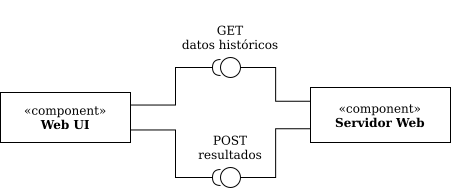
\includegraphics[width=\linewidth]{images/Interfaces web.png}
  \caption{Interfaz de servidor para guardar y recuperar datos históricos de ejecución.}
  \label{fig:diagrama_datos_web}
\end{figure}

Esta página también permite observar los datos recuperados, dando promedios de
tiempo de ejecución para cada microbenchmark y permitiendo filtrar los
resultados a tomar en cuenta basado en plataforma de ejecución y hardware.

\section{Resultados}

Los resultados de este proyecto se centran en la creación de una
infraestructura integral para realizar microbenchmarks en GPUs a través de
múltiples plataformas, utilizando estándares modernos como WebGPU. Cada
componente desarrollado busca abordar las necesidades identificadas en los
objetivos del proyecto y resolver las limitaciones detectadas en herramientas
existentes. A continuación, se describen los principales productos
desarrollados y sus características.

\subsection{Biblioteca uwgpu}

El principal producto técnico del proyecto es la biblioteca “uwgpu”, diseñada
para simplificar el proceso de crear microbenchmarks con la API gráfica WebGPU.
La biblioteca abstrae los detalles técnicos de bajo nivel, permitiendo a los
desarrolladores enfocarse en la implementación de sus algoritmos de prueba.
Mediante una interfaz modular, uwgpu facilita:

\begin{itemize}
	\item La creación y configuración de pipelines computacionales.
	\item La ejecución repetida de operaciones para obtener medidas precisas de rendimiento.
	\item La generación de resultados en un formato estándar, adecuado para análisis posteriores.
\end{itemize}

\subsubsection{Fortalezas}
\begin{itemize}
	\item Multiplataforma: Permite ejecutar microbenchmarks en entornos web y nativos, manteniendo una implementación unificada.
	\item Simplicidad: Reduce la necesidad de escribir código repetitivo, agilizando el desarrollo de pruebas.
\end{itemize}

\subsubsection{Debilidades}
\begin{itemize}
  \item Pruebas son muy aisladas: Aunque funcional, la biblioteca al ser simple
    ejecuta las pruebas en un entorno sencillo, lo cual puede que no refleje de
    la mejor manera un pipeline de un producto real. No cuenta con
    funcionalidad para simular entornos más complejos o integrados en pipelines
    más complejos.
\end{itemize}

\subsection{Banco de microbenchmarks}

Se desarrolló un banco de microbenchmarks que evalúa dos áreas clave:
\begin{enumerate}
\item Operaciones computacionales comunes, como multiplicación matricial,
  convolución, reducción y suma de prefijos (o scan).
\item Operaciones de memoria, incluyendo transferencia de datos entre buffers y
  texturas.
\end{enumerate}

El diseño modular de estos benchmarks permite su integración directa con la
biblioteca “uwgpu”, ofreciendo soporte tanto para entornos web como nativos.
Cada benchmark puede configurarse para ajustar parámetros como el tamaño de los
“workgroups” y el número de iteraciones.

\subsubsection{Fortalezas}

\begin{itemize}
	\item Cobertura: Abarca operaciones fundamentales tanto para computación como
    para gráficos.
	\item Portabilidad: Compatible con navegadores modernos y sistemas operativos
    populares.
\end{itemize}

\subsubsection{Debilidades}
\begin{itemize}
  \item Estandarización: Aunque funcional, el banco carece de validación formal
    frente a estándares reconocidos, lo que podría limitar su uso como
    referencia académica o industrial.
\end{itemize}

\subsection{Herramienta CLI}

La interfaz de línea de comandos (CLI) ofrece un medio eficiente para ejecutar benchmarks en entornos nativos. Esta herramienta permite:
\begin{itemize}
	\item Seleccionar y ejecutar cualquier benchmark del banco previamente desarrollado.
	\item Configurar parámetros específicos como el tamaño de los “workgroups” directamente desde la terminal.
\end{itemize}

\subsubsection{Fortalezas}
\begin{itemize}
	\item Flexibilidad: Ideal para usuarios avanzados y entornos de automatización.
	\item Compatibilidad: Diseñada para sistemas operativos modernos, incluyendo Linux, macOS y Windows.
\end{itemize}

\subsubsection{Debilidades}
\begin{itemize}
	\item Curva de aprendizaje: Requiere conocimientos técnicos básicos para su uso.
\end{itemize}

\subsection{Interfaz Web}

El servidor web desarrollado permite a los usuarios ejecutar benchmarks
directamente desde su navegador. Los resultados de las ejecuciones se almacenan
en una base de datos centralizada, lo que habilita:
\begin{itemize}
	\item La creación de un repositorio de datos históricos de rendimiento.
	\item La visualización y análisis de resultados filtrando los resultados basado
    en plataforma y/o hardware.
\end{itemize}

Esta interfaz democratiza el acceso al benchmarking, permitiendo que usuarios
con hardware diverso contribuyan al análisis colectivo.

\subsubsection{Fortalezas}
\begin{itemize}
	\item Accesibilidad: No requiere instalación previa ni conocimientos avanzados
    para su uso.
	\item Colaboración: Promueve la creación de un banco de datos amplio y diverso,
    útil para análisis estadísticos.
\end{itemize}

\subsubsection{Debilidades}
\begin{itemize}
  \item Limitaciones del navegador: La dependencia de WebGPU podría restringir
    el soporte en navegadores no compatibles, como por ejemplo versiones
    antiguas de Safari.
\end{itemize}

\section{Conclusiones}

En resumen, este proyecto generó los siguientes productos:

\begin{enumerate}
 \item Biblioteca de fuente abierta para escribir microbenchmarks multiplataformas con wgpu.
 \item Biblioteca de banco de microbenchmarks con 7 microbenchmarks implementados para operaciones computacionales comunes y rendimiento de memoria de GPU.
 \item Herramienta CLI para ejecución nativa.
 \item Página web para ejecución en navegador, recolección de datos y visualización de datos.
\end{enumerate}

En general se cuenta con una infraestructura muy completa para evaluación de
microbenchmarks y rendimiento de craracterísticas claves de GPU en todas las
plataformas principales populares. Así como infraestructura para la recolección
de datos y despliegue de una página web para alcanzar usuarios que proporcionen
datos fácilmente.

La principal debilidad de estos resultados es que la falta de estandarización
de las operaciones creadas para microbenchmarks significa que de momento los
resultados generados no son necesariamente útiles para los entornos serios
académicos o industriales.

Adicionalmente otra limitante es que no se contempló recolectar datos de
ejecuciones en entornos nativos para la base de datos. Esto no fue contemplado
por dos razones, la primera es que el proyecto iba más enfocado a las
plataformas web, la herramienta CLI se agregó al alcance en parte por su
facilidad de implementación; la segunda razón es que es menos accesible pedir a
los usuarios que instalen una herramienta CLI para ejecutar los
microbenchmarks, entonces debería de diseñarse una manera amistosa con el
usuario de guiarlos a raelizar la instalación y ejecución fácilmente si esto se
fuese a realizar.

\section{Recomendaciones}

A partir del desarrollo de este proyecto, se identifican las siguientes áreas
de mejora y posibles trabajos futuros para ampliar el alcance, la utilidad y la
aceptación de µwgpu en entornos académicos e industriales:

\subsection{Definición de benchmarks valiosos y estándares modernos}

Es fundamental obtener la asesoría de expertos en gráficos computacionales,
optimización paralela, microarquectura y diseño de algoritmos de GPUs. Esto permitiría:

\begin{itemize}
    \item Identificar qué microbenchmarks serían más relevantes y valiosos, tanto
      para estudios académicos como para aplicaciones industriales.
    \item Priorizar operaciones que puedan proporcionar información clave sobre
      el rendimiento de las GPUs en aplicaciones reales, enfocándose en
      características de memoria y rendimiento computacional críticas.
\end{itemize}

Este criterio experto asegurará que las herramientas desarrolladas estén al nivel
que requiere la comunidad de investigación y la industria, elevando la relevancia
del proyecto.

\subsection{Optimización de operaciones}

Las operaciones implementadas hasta ahora podrían beneficiarse de un análisis
exhaustivo de optimización, utilizando técnicas reconocidas para maximizar el
rendimiento. Esto incluye:

\begin{itemize}
    \item Adaptar las implementaciones para utilizar prácticas modernas para
      asegurar que las operaciones optimizadas estén alineadas con los estándares
      más avanzados y reflejen el estado del arte en la optimización de GPU.
    \item Validar las optimizaciones mediante herramientas como perfiles de GPU
      y comparativas con benchmarks de referencia.
\end{itemize}

Esto aumentara el valor práctico de los resultados generados ya que podrán ser
comparados con los resultados de otras investigaciones o con el rendimiento
de una aplicación seria de producción.

\subsection{Recolección de datos en entornos nativos}

Para ampliar la utilidad del proyecto, se recomienda incluir soporte para la
recolección de datos desde ejecuciones nativas, complementando los datos
obtenidos en navegadores. Esto requeriría:

\begin{itemize}
    \item Diseñar una solución simplificada para que los usuarios descarguen e
      instalen la herramienta CLI, facilitando su uso. Se propone posiblemente
      mediante un único comando que automatice la instalación y ejecución de
      los benchmarks.
    \item Desarrollar una guía clara y detallada en la página web del proyecto,
      explicando cómo realizar la instalación y ejecución en los sistemas
      operativos más comunes (Linux, macOS y Windows).
    \item Integrar los resultados recolectados de entornos nativos a la base de
      datos existente, para enriquecer el análisis estadístico y proporcionar
      una visión más completa del rendimiento multiplataforma.
\end{itemize}

Estas mejoras no solo incrementarían la accesibilidad del proyecto, sino que
también diversificarían los datos recolectados, aumentando su relevancia y
aplicabilidad.

\nocite{*}
\printbibliography


\end{document}
